\section{Architecture and Implementation}

Until now, this paper has been primarily concerned with the details of the
CSlang language.  However, the language alone is not enough to do the work
we intended it to accomplish.  The CSlang tool set
consists of several related
components that allow a CSlang program to be used to analyze a stream of
application activity.
In this section we discuss the most important of these components and some
of the decisions that went into their design and operation.

\label{SEC:architecture}

\begin{figure}
  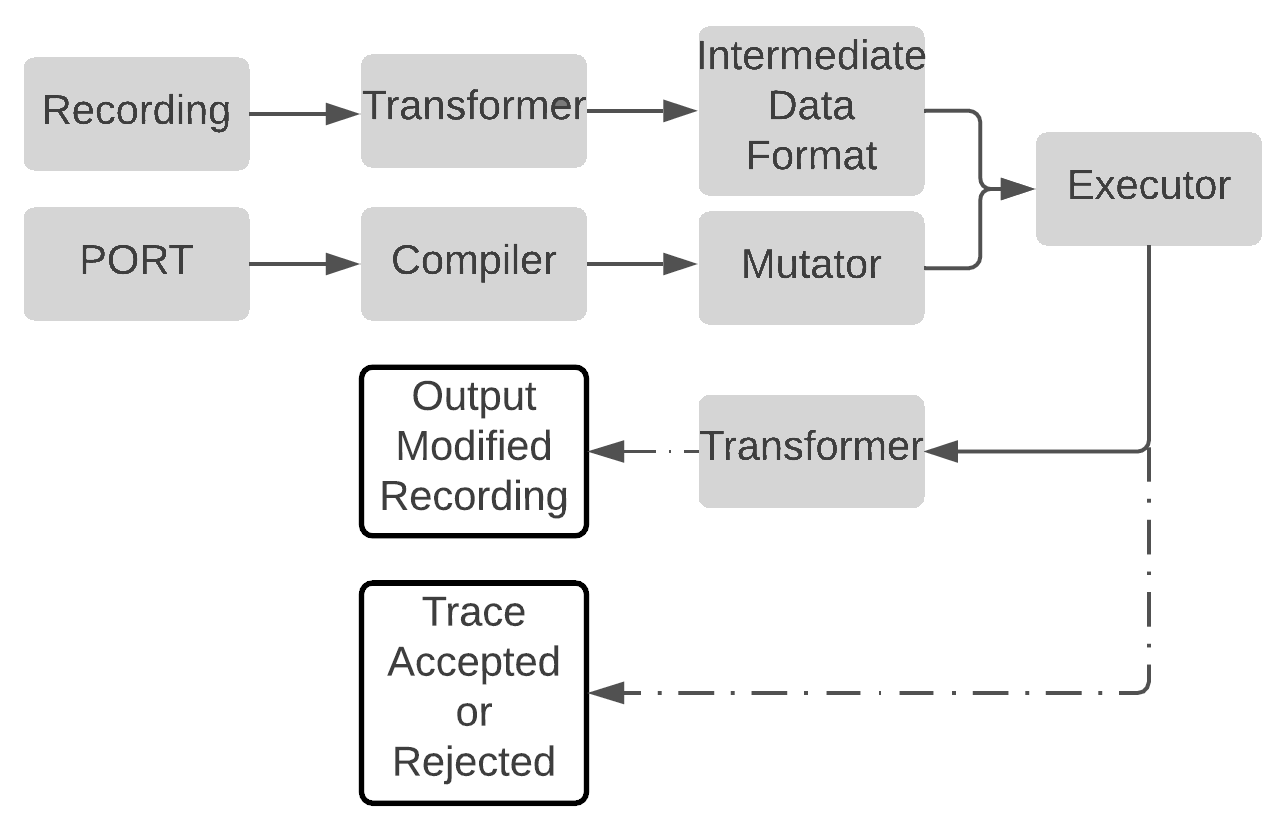
\includegraphics[scale=.08]{images/architecture}
  \caption{The CSLang compiler produces a Mutator that operates over a
  generic internal data format that contains the contents of an application
  recording.}
  \label{fig:architecture}
\end{figure}

\subsection{The CSlang Compiler}

The CSlang compiler is responsible for constructing a Mutator
from a description contained in  a CSlang program.
We made the decision to make CSlang a compiled language because
the earlier SEA work showed that CSlang programs are typically
compiled a few times during construction
and executed many times over many different applications.
By compiling ahead of time we save the performance cost associated with other
approaches like just-in-time compilation or execution via an interpreter.
Compilation happens in two phases.  In the first phase, the program text is
parsed into an abstract syntax tree using an LALR parser.
In the second, the
contents of the AST are used to assemble a complete Mutator.
This Mutator is serialized to
disk so that it may be stored and reused.


\subsection{The Internal Data Format}

We wanted to make CSlang flexible
to take the SEA technique beyond system calls
so it could
work with many different sorts of
activity representations.
This required a method to cleanly separate the details of how
an application's activity was recorded from the representation that will be
processed by a Mutator.
Our solution was twofold.  First, we developed an internal data format
(IDF) that
could store the key components, such as parameter and return values,
for application activities like function
and system calls.  This format supports primitive string and numeric
values as well as arbitrarily nested structures in the form of records.
The decision to include these features
was based on the Linux kernel's system call implementation
which allows system call inputs and outputs in the form of primitive data
values and complex structures.
These capabilities would be necessary
if CSlang was going to support system calls.

The second component is the set of modules, known as transformers, that can
convert an activity stream from its original representation into IDF and
back.  A transformer achieves the former by parsing each activity entry,
extracting the relevant fields, and assembling this information into an IDF
record.  These records are re-assembled into a stream which is input into a
Mutator.
The output generated by processing this input stream
is converted by a transformer
back into the original activity representation.

\subsection{Executing a CSlang Program}

Unlike an executable program, a compiled CSlang program is a static entity
that cannot run by itself.  Instead, a component we refer to as the
``CSlang Executor'' is responsible for carrying out the ancillary work
required to analyze an application recording with a Mutator.
These tasks include deserializing a stored Mutator from a disk,
converting the selected input stream
to CSlang's internal data format
using an appropriate transformer,
translating the output stream back to the original activity representation,
and reporting whether the input sequence was
accepted or rejected by the Mutator.

\subsection{Nuts and Bolts}

